\documentclass{article}
\usepackage{amsmath, amssymb, cite, algorithmic, url, braket}
\usepackage{graphicx}
\usepackage{pythonhighlight}
\usepackage[margin=1.5cm]{geometry}
\usepackage[title]{appendix}
\usepackage{subfigure}
\usepackage{listings}
\usepackage{booktabs}
\usepackage{hyperref}

\graphicspath{{../pic/}}
\lstset{
language=[ANSI]{C},
showtabs=true,
tab=,
tabsize=2,
basicstyle=\ttfamily\footnotesize,%\setstretch{.5},
stringstyle=\color{stringcolour},
showstringspaces=false,
alsoletter={1234567890},
otherkeywords={\%, \}, \{, \&, \|},
keywordstyle=\color{keywordcolour}\bfseries,
upquote=true,
morecomment=[s]{/*}{*/},
commentstyle=\color{commentcolour}\slshape,
literate=*%
{=}{{\literatecolour=}}{1}%
{-}{{\literatecolour-}}{1}%
{+}{{\literatecolour+}}{1}%
{*}{{\literatecolour*}}{1}%
{!}{{\literatecolour!}}{1}%
{[}{{\literatecolour[}}{1}%
{]}{{\literatecolour]}}{1}%
{<}{{\literatecolour<}}{1}%
{>}{{\literatecolour>}}{1}%
% {>>>}{\pythonprompt}{3}%
,%
frame=trbl,
rulecolor=\color{black!40},
backgroundcolor=\color{white},
breakindent=.5\textwidth,frame=single,breaklines=true
}

\begin{document}
\title{DSP Monthly Project 3}
\author{Xu, Minhuan}
\maketitle
\tableofcontents
\begin{abstract}
Using a guitar tuner on a mobile phone has to face a difficult graphical interface and endless advertisements, so I wrote a command line tuner using python. Its judgement of overtones is not accurate, but the judgement of high strings is mature.
\end{abstract}


\section{Process}
\subsection{Reason}
When I play the guitar at ordinary times, I always find that I don't have a guitar tuner beside me. In this case, we always use the software on the phone to tune. This is a convenient method, but it is always bothered by endless advertisements. So I want to use Python to write a tuner on a computer that can provide real-time feedback.
\subsection{Implement}
I will put my code in the appendix, which uses spectrum analysis to find the current playing method, but I also encountered some problems. For example, the overtone of a guitar affects the pitch resolution in the spectrum. Because the spectrum of the pitch is not too wide, I use the interval between overtones to indicate the frequency of the tone. At the same time, if the resolution is too high, the spectrum of a single sound will become wider, so I reduced the resolution to make the spectrum more readable for both humans and computers.
\section{Result}
\subsection{Terminal Output}
Please take a look at the screenshot of my use.
\begin{figure}[!h]
	\centering
	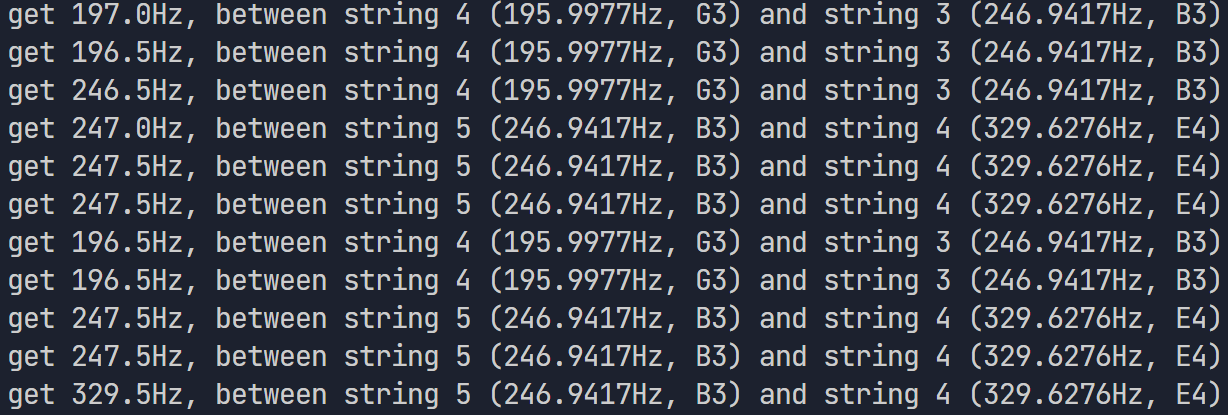
\includegraphics[width=3 in]{../pic/out1.png}
	\caption{Terminal Output When Tuning Different Strings}
	\label{fig:output}
\end{figure}
\subsection{My Future Vision}
Judging overtones by the method in the code I wrote is not yet mature, because the points near the same frequency will occupy the first three of the amplitude comparison, which leads to the failure of extracting overtones correctly, and the method of judging the pitch by the difference of overtones may fail. However, if there is no overtone in the frequency band of the guitar, such as the last three strings, it will not lead to misjudgment and improve the accuracy.

So if I want to improve this tuner in the future, I will first let the user select the string to be calibrated, so as to avoid misjudgment between different strings; Or if I learn the method of extracting pitch in the future, I will find the tuner and write the code.


\bibliographystyle{ieeetr}
\bibliography{../bib/database}

\begin{appendices}
\section{Code Listing}
\begin{python}
import pyaudio
import numpy as np 
from scipy import signal
import matplotlib.pyplot as plt
from time import sleep

FORMAT = pyaudio.paInt16 # Bit depth
CHANNELS = 1 # 1 channel
SAMPLE_RATE = 3000  # sample rate fs
SAMPLE_INTERVAL = 1/SAMPLE_RATE # 1/fs
T = 2 # Duration of a short audio segment (s)
RES = 1./T # Resolution of tuner (Hz)
CHUNK = T*SAMPLE_RATE # The number of sampling points

lowcut, highcut = 75.0, 1250.0 # Bandpass
freq_range = [75, 350] # The Frequency Range of Guitar Strings
freq = np.fft.rfftfreq(CHUNK, d=SAMPLE_INTERVAL) 
mask = (freq < freq_range[0]) + (freq > freq_range[1])

# Notes and frequencies corresponding to six strings
Notes_guitar = ['E2','A2','D3','G3','B3','E4']
freq_guitar = np.array([82.4069, 110.0000, 146.8324,
                        195.9977, 246.9417, 329.6276])

# Initialize microphone input
p = pyaudio.PyAudio()
in_stream = p.open(format=FORMAT, channels=CHANNELS, rate=SAMPLE_RATE,\
                input=True, frames_per_buffer=CHUNK)

for i in range(10):  
    buffer = in_stream.read(CHUNK, exception_on_overflow = False)
    y = np.frombuffer(buffer, dtype = np.int16)
    # real number fft
    Y = np.fft.rfft(y)/CHUNK
    Y_a = np.abs(Y)

    # Bandpass filter
    sos = signal.butter(10, [lowcut, highcut], 'bp', fs=SAMPLE_RATE, output='sos')
    filtered = signal.sosfilt(sos, y)
    FILTERED = np.fft.rfft(filtered)/CHUNK
    FILTERED_a = np.abs(FILTERED)
    
    S_a = FILTERED_a
    S_a[mask] = 0 # Noise removal
    freq_max = np.argmax(S_a)
    main_freq = freq[freq_max] # Find the frequency with the largest amplitude
    S_a[freq_max] = 0
    freq_max = np.argmax(S_a)
    second_freq = freq[freq_max]
    base_freq = main_freq - second_freq
    if (np.abs(main_freq - second_freq) > 75):
        main_freq = np.abs(base_freq)

    NoString = 0
    for i in range(6):
        if main_freq > freq_guitar[i]:
            NoString += 1
        else:
            break
    if NoString == 0:
        message = f"get {main_freq}Hz, lower than string 6 ({freq_guitar[NoString]}Hz, {Notes_guitar[NoString]})"
    elif NoString == 6:
        message = f"get {main_freq}Hz, higher than string 1 ({freq_guitar[NoString]}Hz, {Notes_guitar[NoString]})"
    else:
        message = f"get {main_freq}Hz, between string {NoString} ({freq_guitar[NoString-1]}Hz, {Notes_guitar[NoString-1]}) and string {NoString-1} ({freq_guitar[NoString]}Hz, {Notes_guitar[NoString]})"
    print(message)
    sleep(1)
\end{python}
\end{appendices}

\end{document}